\documentclass{article}

\usepackage{amsmath, amssymb}
\usepackage{float}
\usepackage{graphicx}
\usepackage{subcaption}
\usepackage{color}
\usepackage[table,xcdraw]{xcolor}

\usepackage{polski}

\usepackage{listings}


\definecolor{dkgreen}{rgb}{0,0.6,0}
\definecolor{gray}{rgb}{0.5,0.5,0.5}
\definecolor{mauve}{rgb}{0.58,0,0.82}

\lstset{frame=tb,
  language=C++,
  aboveskip=3mm,
  belowskip=3mm,
  showstringspaces=false,
  columns=flexible,
  basicstyle={\small\ttfamily},
  numberstyle=\color{gray},
  keywordstyle=\color{blue},
  commentstyle=\color{dkgreen},
  stringstyle=\color{mauve},
  breaklines=true,
  breakatwhitespace=true,
  tabsize=3,
}
%

\addtolength{\topmargin}{-.875in}
\addtolength{\textheight}{1.75in}


\begin{document}
	\section{Algorytmy}
		\subsection{Przechodzenie między kolorami w klasie Color}
			\begin{lstlisting}
				Color Color::next()
				{
					switch (m_current_cycle)
					{
					case cycle::Gu:
						G += m_step;
						if (G > 255)
						{
							G = 255;
							m_current_cycle = cycle::Rd;
						}
						break;
					case cycle::Rd:
						R -= m_step;
						if (R < 0)
						{
							R = 0;
							m_current_cycle = cycle::Bu;
						}
						break;
					case cycle::Bu:
						B += m_step;
						if (B > 255)
						{
							B = 255;
							m_current_cycle = cycle::Gd;
						}
						break;
					case cycle::Gd:
						G -= m_step;
						if (G < 0)
						{
							G = 0;
							m_current_cycle = cycle::Ru;
						}
						break;
					case cycle::Ru:
						R += m_step;
						if (R > 255)
						{
							R = 255;
							m_current_cycle = cycle::Bd;
						}
						break;
					case cycle::Bd:
						B -= m_step;
						if (B < 0)
						{
							B = 0;
							m_current_cycle = cycle::Gu;
						}
					}
					return *this;
				}
			\end{lstlisting}
			\pagebreak
			W każdym kroku zmienia się jeden ze składników RGB koloru w zależności od etapu na którym jest algorytm i zadanego skoku.
			Algorytm zakłada, że pierwotny kolor to (255, 0, 0) czyli czerwony. Kolejne etapy:
			\begin{enumerate}
				\item G rośnie od 0 do 255,
				\item R spada od 255 do 0,
				\item B rośnie od 0 do 255,
				\item G spada od 255 do 0,
				\item R rośnie od 0 do 255,
				\item B spada od 255 do 0.
				\item Przejście do kroku 1.
			\end{enumerate}
			\begin{figure}[h!]
				\centering
				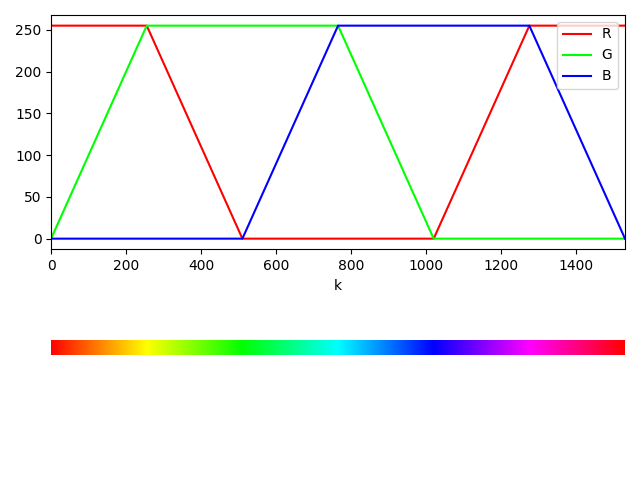
\includegraphics[width = \textwidth]{img/colors}
				\caption{Wartości składników RGB w kolejnych krokach działania algorytmu wraz z odpowiadającymi im kolorami.}
			\end{figure}
		\subsection{Generowanie odcinków krzywej w klasie CurveGenerator}
			\begin{lstlisting}
				Segment CurveGenerator::generate_segment()
				{
					Point start = m_curve.get_pos(m_t, m_is_cartesian);
					double current_segment_length = 0;
					Point pos;
					int i = 0;
					while (current_segment_length < m_segment_length && i < 400)
					{
						i++;
						pos = m_curve.get_pos(m_t += m_segment_generation_step, m_is_cartesian);
						current_segment_length = sqrt(pow(start.x - pos.x, 2) + pow(start.y - pos.y, 2) + pow(start.z - pos.z, 2));
					}
					return Segment(start, pos, color.next());
				}
			\end{lstlisting}
			Po ustaleniu położenie krzywej dla argumentu $t$, szukany jest odcinek o zadanej długości poprzez stopniowe zwiększanie parametru $t$.
			Poszukiwanie zostaje przerwane jeżeli zostanie znaleziony odcinek o pożądanej długości lub przekroczona zostanie maksymalna liczba iteracji (tu: 400).
		\subsection{Generowanie krzywej w klasie CurveGenerator}
			\begin{lstlisting}
				std::deque<Segment> CurveGenerator::get_next()
				{
					if (m_animate)
					{
						Segment seg = generate_segment();
				
						if (m_current_segment_count > m_max_animation_segment_count)
						{
							m_queue.pop_front();
						}
						else
							m_current_segment_count++;
				
						m_queue.push_back(seg);
				
						for (int i = 0; i < m_current_segment_count - 0.6 * m_max_animation_segment_count; i++)
							m_queue[i].color += (int)(255.0 / (0.4 * m_max_animation_segment_count));
				
						return m_queue;
					}
					else
					{
						while (m_current_segment_count < m_max_segment_count)
						{
							m_current_segment_count++;
							Segment seg = generate_segment();
							m_queue.push_back(seg);
						}
					}
					return m_queue;
				}
			\end{lstlisting}
			W zależności od tego czy krzywa ma być animowana czy nie, algorytm zachowuje się w różny sposób.
			W pierwszym przypadku kolejne segmenty dokładane są tak długo, aż nie zostanie osiągnięty ich limit. Wtedy w każdej iteracji poza dodaniem nowego segmentu jednocześnie usuwany jest najstarszy segment należący do krzywej.
			Jednocześnie, jeżeli długość krzywej zacznie przekraczać 60\% maksymalnej długości, najstarsze segmenty zostają stopniowo rozjaśniane.
			Jeżeli krzywa nie jest animowana, funkcja generuje po prostu całość krzywej na raz.
\end{document}